\chapter{Analysis}
\label{analysis}

To verify \dcamp meets both the transparency and scalability distributed performance framework criterion outlined in
Chapter \ref{introduction}, several experiments were run on an installation of \dcamp in a test environment. The goal of
these experiments was two fold: measure \dcampns's transparency in a real-world environment as well as determine the
thresholds for several key configuration parameters as \dcamp scales.

Any DPF can be configured in such a way that it impacts the performance of the system being monitored, for example by
collecting and reporting every available global metric and per-process metrics at the fastest sampling period.
Therefore, it is necessary for the system administrator to know what reasonable configuration values should be used to
monitor a given distributed system.

Likewise, for \dcamp to scale, it is important for the number of child nodes per parent to be limited to a reasonable
number. These experiments help to define ``reasonable'' for various scenarios, environments, and performance monitoring
requirements.

\section{Transparency}

To measure the impact of \dcamp on a monitored process, a workload is defined and measured with and without \dcamp
active. The measured difference in performance of the monitored process is defined to be \dcampns's monitoring overhead.

\subsection{Workload}

Apache JMeter\cite{jmeter} (v2.11) is used to run load against a default-configured Apache instance on a Lenovo Thinkpad
(dual 2.16GHz Centrino Duo T2600, 2GB 667MHz DDR2, SATA) running Ubuntu 13.10. The client machine, a MacBook Pro (2.7GHz
Core i7, 8GB 1333MHz DDR3, SSD) running OSX 10.9, is directly connected to the Apache server via crossover gigabit
Ethernet.

Each test run includes 18 different load points, scaling the number of client threads from 2 to 2048. For every load
point, the threads continuously (in this order)

\begin{enumerate}
\item load a static home page,
\item load a PHP page which calculates the 25th Fibonacci number (see Figure \ref{fig:fib25_list}), and
\item download a 5MB file of random binary data.
\end{enumerate}

The 25th Fibonacci workload is CPU-bound, and the 5MB download is disk-bound; the home page workload is only used to
seed the client connection and is not part of the analysis measurements. After the ramp up phase of each load point
(launching 10 threads per second), the test ensures all threads continue to execute simultaneously for five minutes
before shutting down.

The arithmetic mean of the request latency for each step at each load point is then calculated and averaged across three
distinct runs of the same test.

\begin{figure}[H]
\vspace{+10pt}
\begin{lstlisting}[language=php,frame=single,basicstyle=\footnotesize\ttfamily]
<?php
function F($n) {
    if ($n == 0) { return 0; }
    if ($n == 1) { return 1; }
    return F($n - 1) + F($n - 2);
}
?>
<html>
  <body>The 25th Fibonacci number is <?= F(25) ?>.</body>
</html>
\end{lstlisting}
\vspace{-10pt}
\caption[Recursive 25th Fibonacci PHP Script]
	{Recursive 25th Fibonacci PHP Script: A naive approach was used in the implementation of \texttt{F()} in order
	 to put more load on the server CPU.}
\label{fig:fib25_list}
\end{figure}

\subsection{\dcamp Configuration}

Each \dcamp configuration level monitors four global metrics and three process-specific metrics on the Apache
process(es). The global metrics are CPU usage (\texttt{proc}), memory usage (\texttt{mem}), disk throughput
(\texttt{disk}), and network throughput (\texttt{net}); the Apache metrics are CPU usage (\texttt{apache\_cpu}), memory
usage (\texttt{apache\_mem}), and combined disk/network throughput (\texttt{apache\_io}). Below are the various sample
periods used for the transparency test runs.

\begin{itemize}
\item \textbf{baseline} -- \dcamp off
\item \textbf{5m} -- all metrics every 300 seconds, heartbeats every 60 seconds
\item \textbf{1m} -- all metrics every 60 seconds, heartbeats every 60 seconds
\item \textbf{10s} -- global metrics every 300 seconds, Apache metrics every 10 seconds, heartbeats every 300 seconds
\item \textbf{1s} -- global metrics every 300 seconds, Apache metrics every 1 second, heartbeats every 300 seconds
\end{itemize}

No thresholds were defined for any of the above configurations. That is, Sensor nodes immediately reported every sample
instead of holding them for later reporting.

\subsection{Results}

In the CPU-bound Fibonacci test, the biggest relative increase in request latency occurs between the runs with two and
four threads. This correlates to the two physical CPU cores on the system exceeding capacity. The 1m config run exhibits
the worst performance of all the CPU-bound tests. This shows that global metric monitoring is actually more CPU
intensive than collecting per-process metrics, even for processes with many active processes.

The rate at which request latency worsens begins to level off starting at the 512 thread load point. This is also the
load point at which Apache begins to return errors. As the percentage of requests resulting in errors increases, the
latency of the successful requests improves slightly. This explains the trend line shift.

\begin{figure}[H]
    \centering
    \vspace{-20pt}
    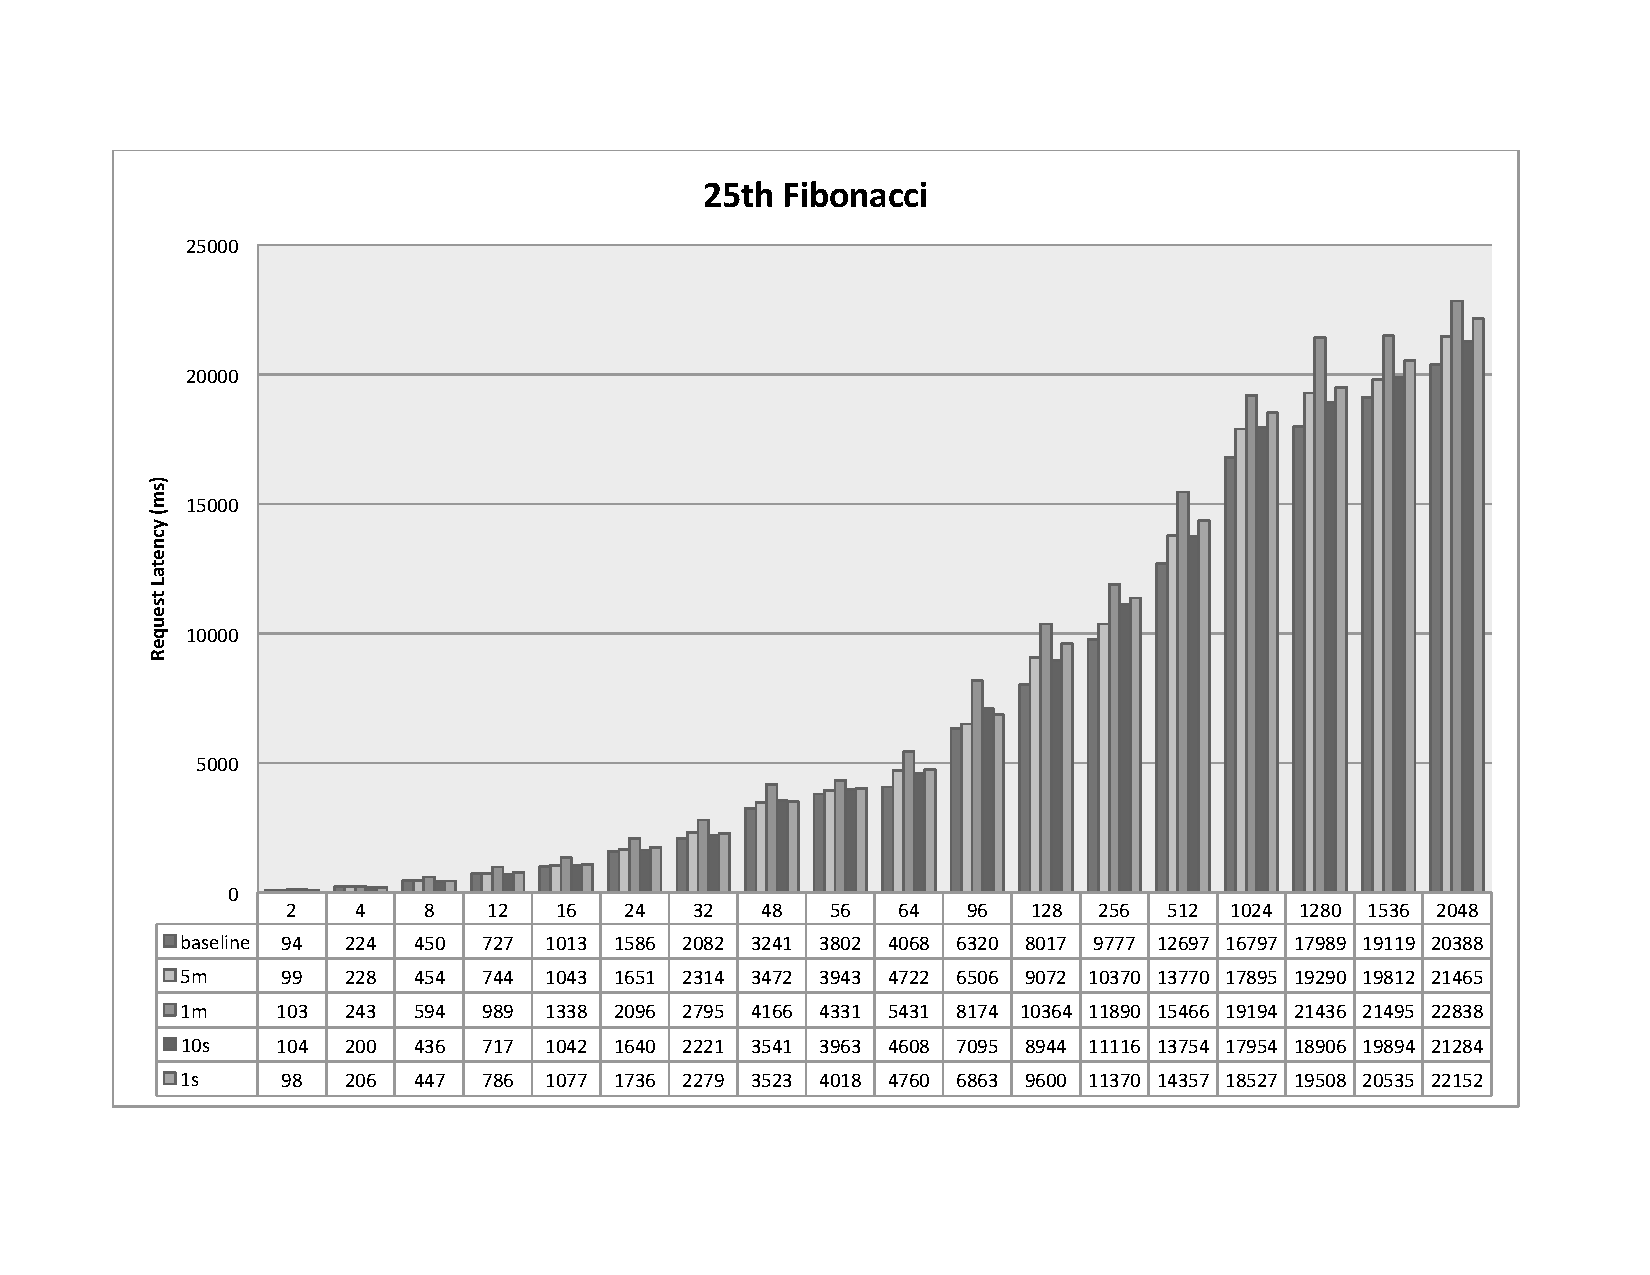
\includegraphics[scale=0.5]{compare-fib.pdf}
    \vspace{-50pt}
    \caption{Transparency: 25th Fibonacci}
    \label{fig:fib25_graph}
\end{figure}

Apache's disk-bound performance measured in the 5MB download test is relatively unaffected by \dcampns. This is expected
since the infrequent samples being logged to an output file are \dcampns's only disk access. This graph also shows the 512
thread load point as the beginning of a trend line shift, again correlating with the increase in request error rate.

\begin{figure}[H]
    \centering
    \vspace{-20pt}
    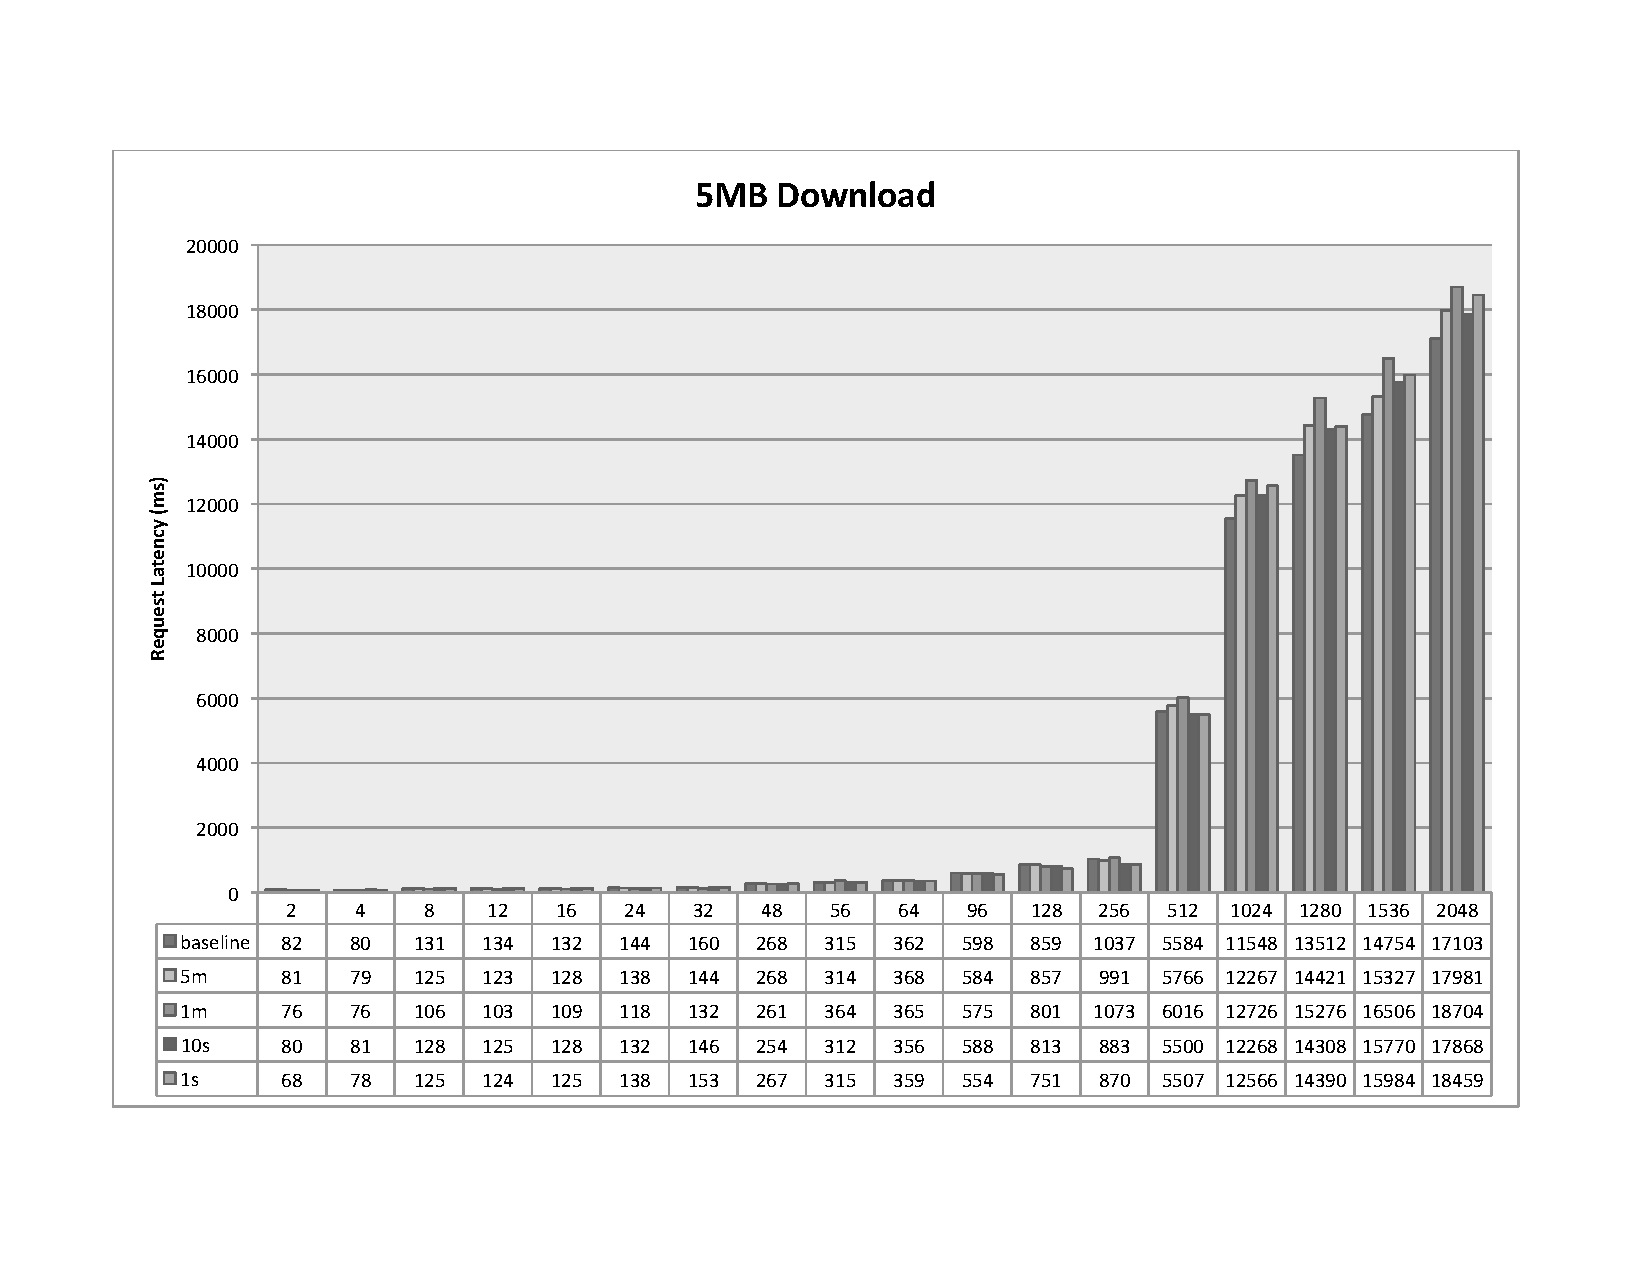
\includegraphics[scale=0.5]{compare-down.pdf}
    \vspace{-50pt}
    \caption{Transparency: 5MB Download}
    \label{fig:down5mb_graph}
\end{figure}

A few observations can be drawn from these results.

When nodes are not expected to fail frequently, using longer heartbeat periods reduces the impact \dcamp has on the
system. It is better to monitor a process using a faster sample period than an entire system using a slower sample
period. The \dcamp system impact is noticeable but a considerably smaller factor than the impact hardware limitations
have on performance monitoring.

Lastly, holding all else constant, slower sample periods have an obviously lower impact on system performance compared
to faster sample periods. Possibly using \dcampns's reporting threshold, system impact can be minimized while still
maintaining fine sample granularity.

\section{Scalability}

One of the primary measures of scalability for a distributed system is its network traffic.\cite{zanikolas2005} By
simulating successively larger \dcamp systems (with respect to node count), one can extrapolate \dcampns's effectiveness
at monitoring large distributed systems and how to best configure its metric collections.

\subsection{Workload}

\dcamp is setup to monitor a machine's global metrics, scaling the number of simulated nodes in the \dcamp system from
three nodes (one \textit{Root}, one \textit{Collector}, one \textit{Metric}) up to 200 nodes (eight groups with
twenty-five nodes per group). The metric configuration is kept constant for each test run. As \dcamp starts, monitors in
steady state, and shuts down, the machine's network traffic is monitored and recorded every five seconds.

The test machine is a MacBook Pro (2.7GHz Core i7, 8GB 1333MHz DDR3, SSD) running OSX 10.9. All simulated \dcamp nodes
use endpoints on the machine's loopback interface, and only the loopback interface traffic is monitored. The machine is
otherwise entirely idle during the test runs.

\subsection{\dcamp Configuration}

\dcamp is configured to monitor and report the below global metrics, using a heartbeat of 60 seconds.

\begin{itemize}
\item CPU usage every 60 seconds
\item total disk throughput every 120 seconds
\item total network throughput every 120 seconds
\item memory usage every 60 seconds
\end{itemize}

No thresholds were defined for the above configuration. That is, Sensor nodes immediately reported every sample instead
of holding them for later reporting.

\subsection{Results}

Sparklines of each load point show the same pattern: highest network traffic occurs during start up and then also on
shutdown. This pattern follows the design of \dcamp which uses a chatty configuration protocol and a terse data
protocol. The rest of steady operation shows expected low network traffic except on sample periods.

\begin{figure}[H]
    \centering
    \vspace{-20pt}
    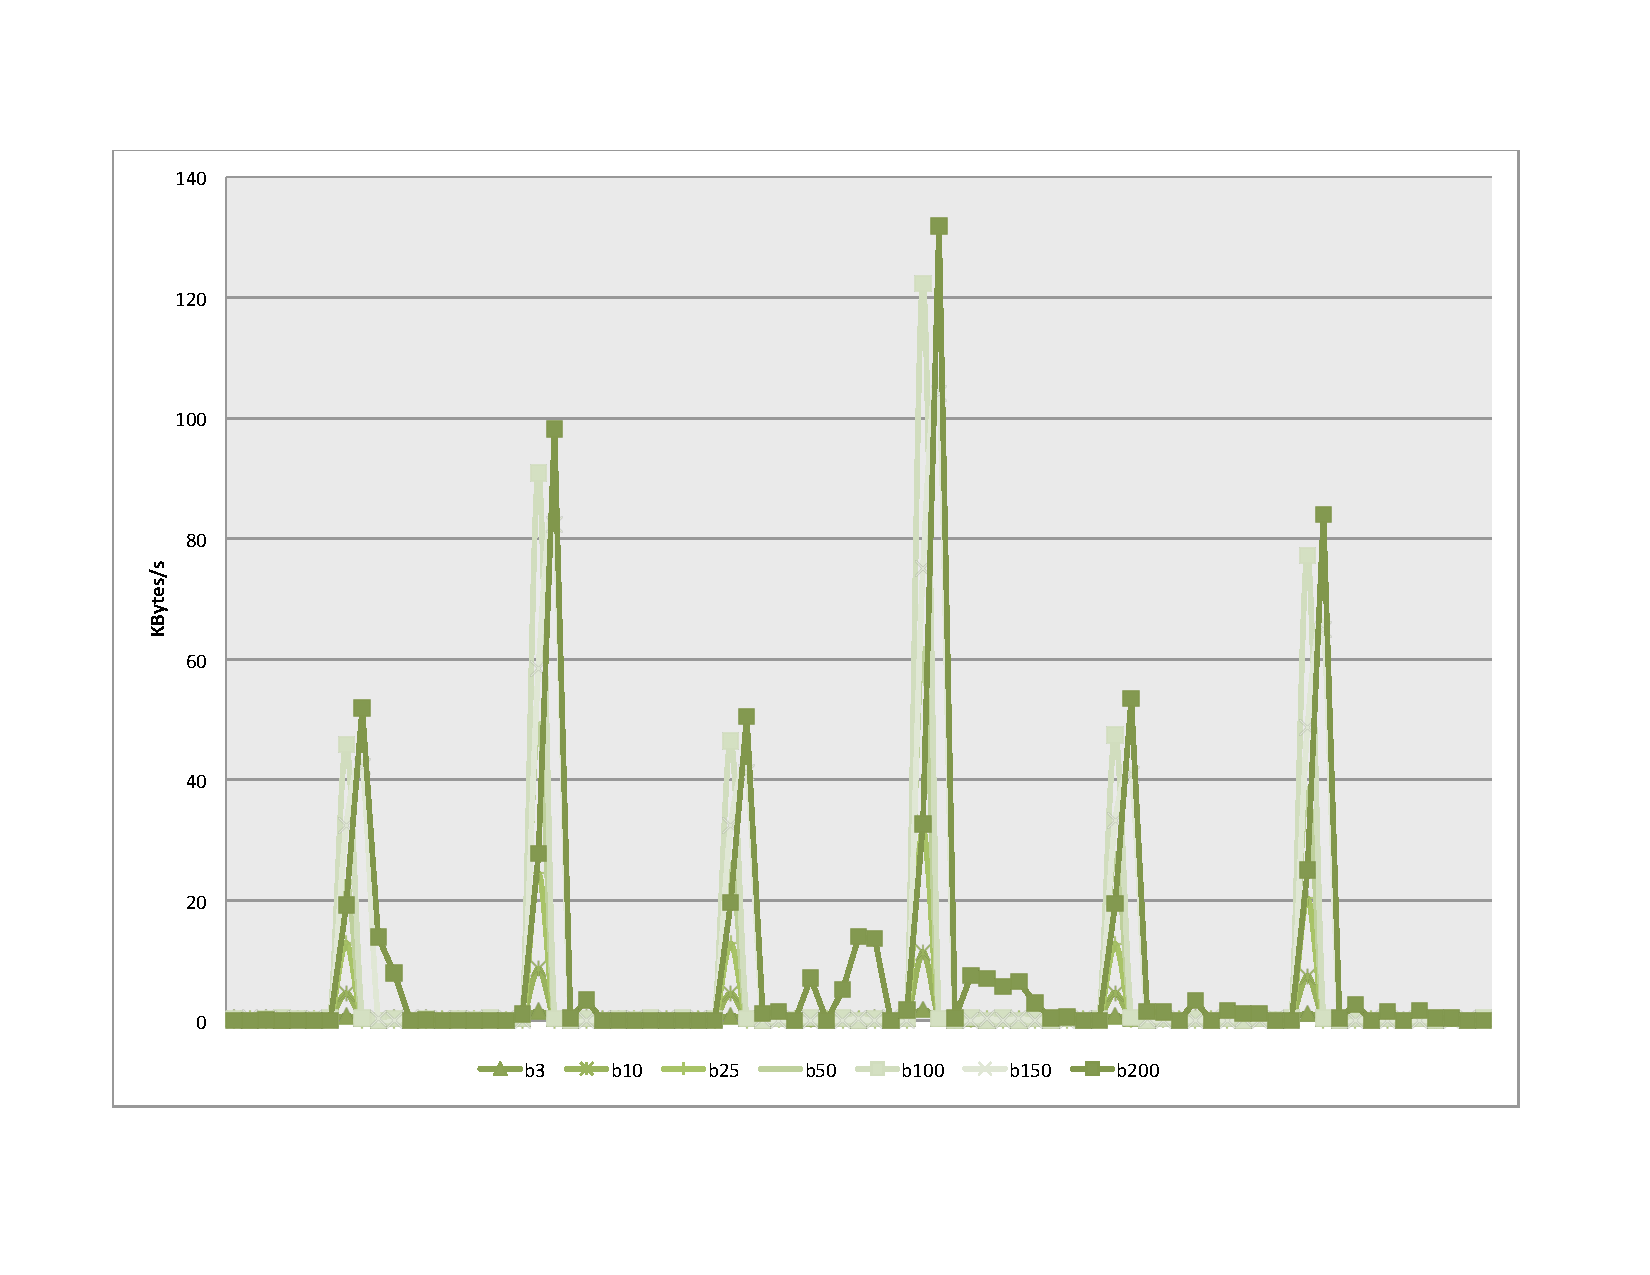
\includegraphics[scale=0.5]{dcamp-net-bytes-steady.pdf}
    \vspace{-40pt}
    \caption[Scalability: Steady State Network Bytes]
            {Scalability: Network bytes during steady operation as the number of \dcamp nodes increases.}
    \label{fig:net_bytes_steady_graph}
\end{figure}

\begin{figure}[H]
    \centering
    \vspace{-20pt}
    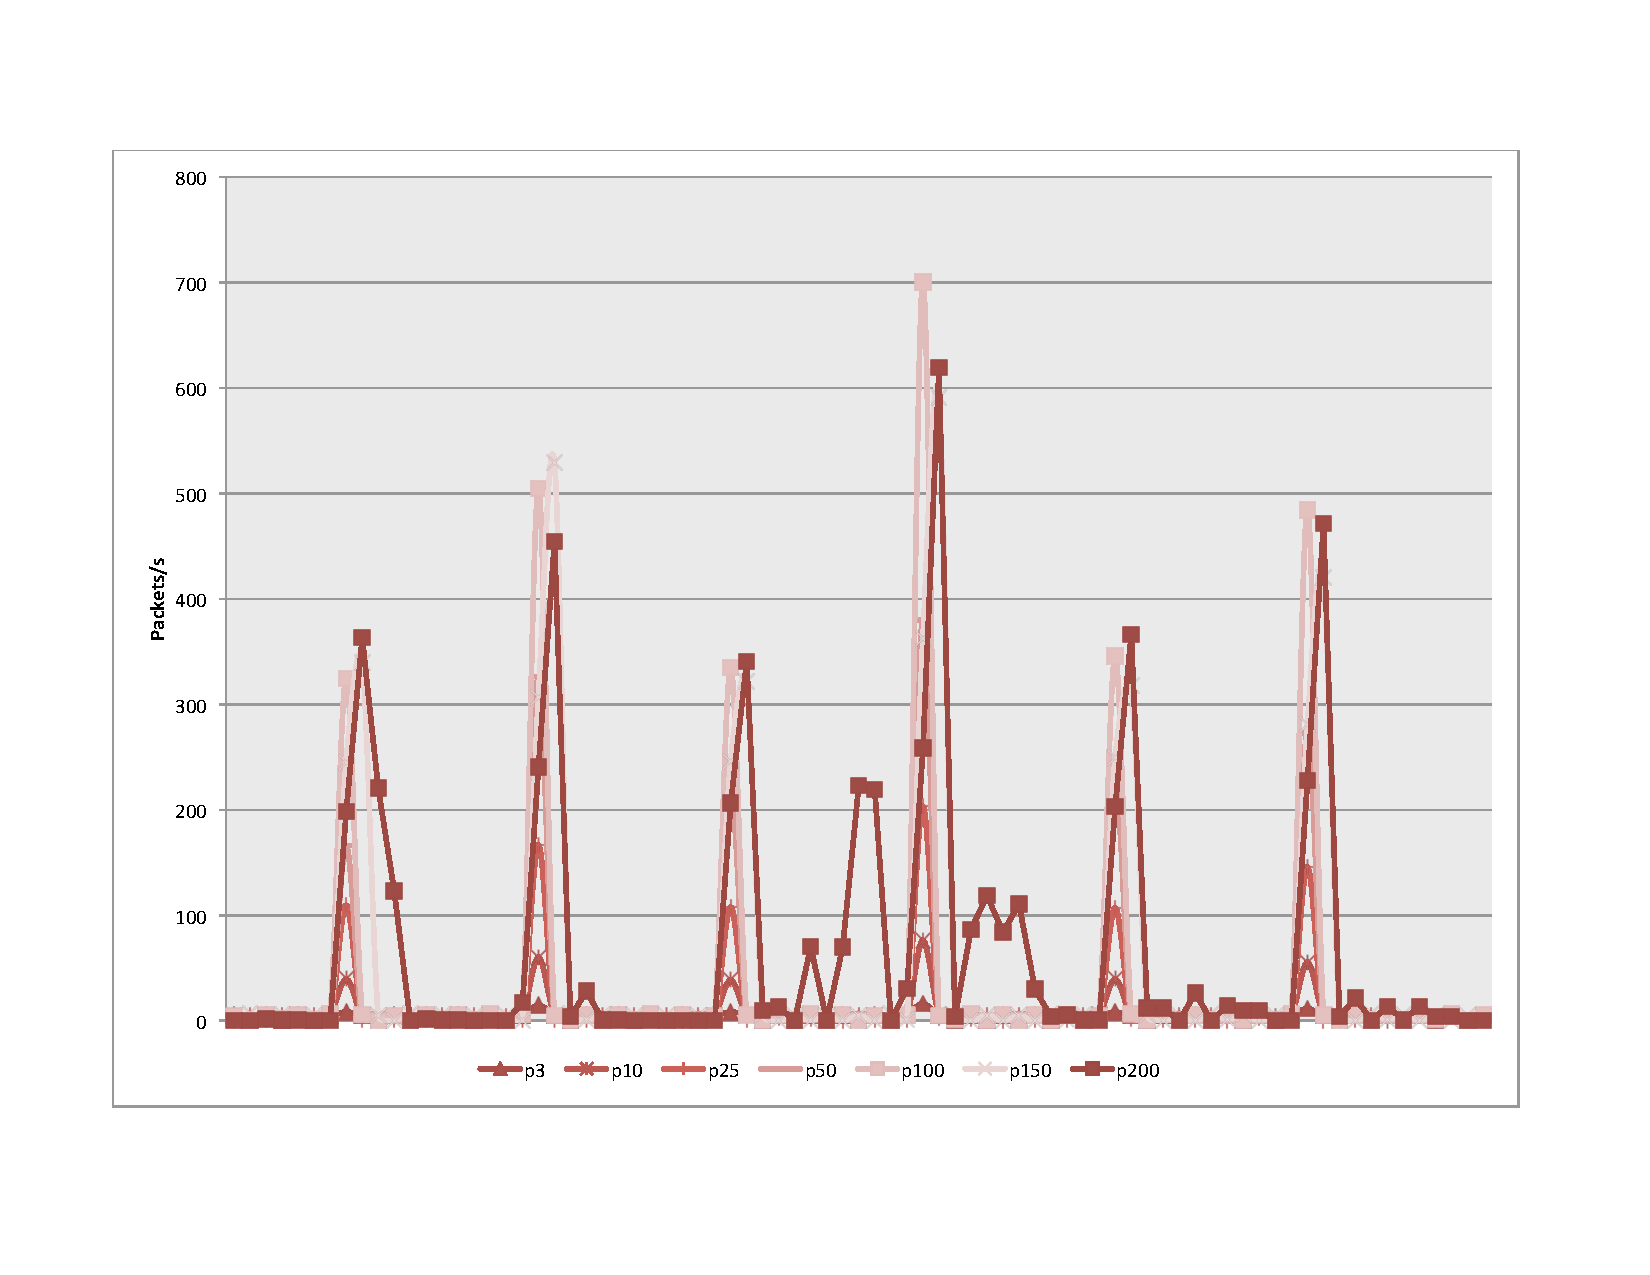
\includegraphics[scale=0.5]{dcamp-net-packets-steady.pdf}
    \vspace{-40pt}
    \caption[Scalability: Steady State Network Packets]
	    {Scalability: Network packets during steady operation as the number of \dcamp nodes increases.}
    \label{fig:net_packets_steady_graph}
\end{figure}

As the node count increases, the rate at which bytes/packets are sent and received increases. This correlates with the
larger configuration which \dcamp must track as well as the additional nodes sending and receiving data. Looking at the
same values but also relating them to the number of nodes in the system, one sees the configuration size grows faster
than the number of nodes.

However, the number of messages being sent per node actually goes down and levels off just under 1 packet per node per
second. This can be attributed to the fact that the number of Sensor nodes increases faster in relation to the number of
\textit{Collector} nodes. That is, Sensor nodes do not require full-configuration replication and send/receive fewer messages
since they are relatively uninvolved with topology coordination in comparison to \textit{Collector} nodes.

As this ratio increases, it is expected the number of messages per node to decrease. This latter observation indicates a
higher number of child nodes per parent would result in lower network utilization and better \dcamp scalability.

\begin{figure}[H]
    \centering
    \vspace{-20pt}
    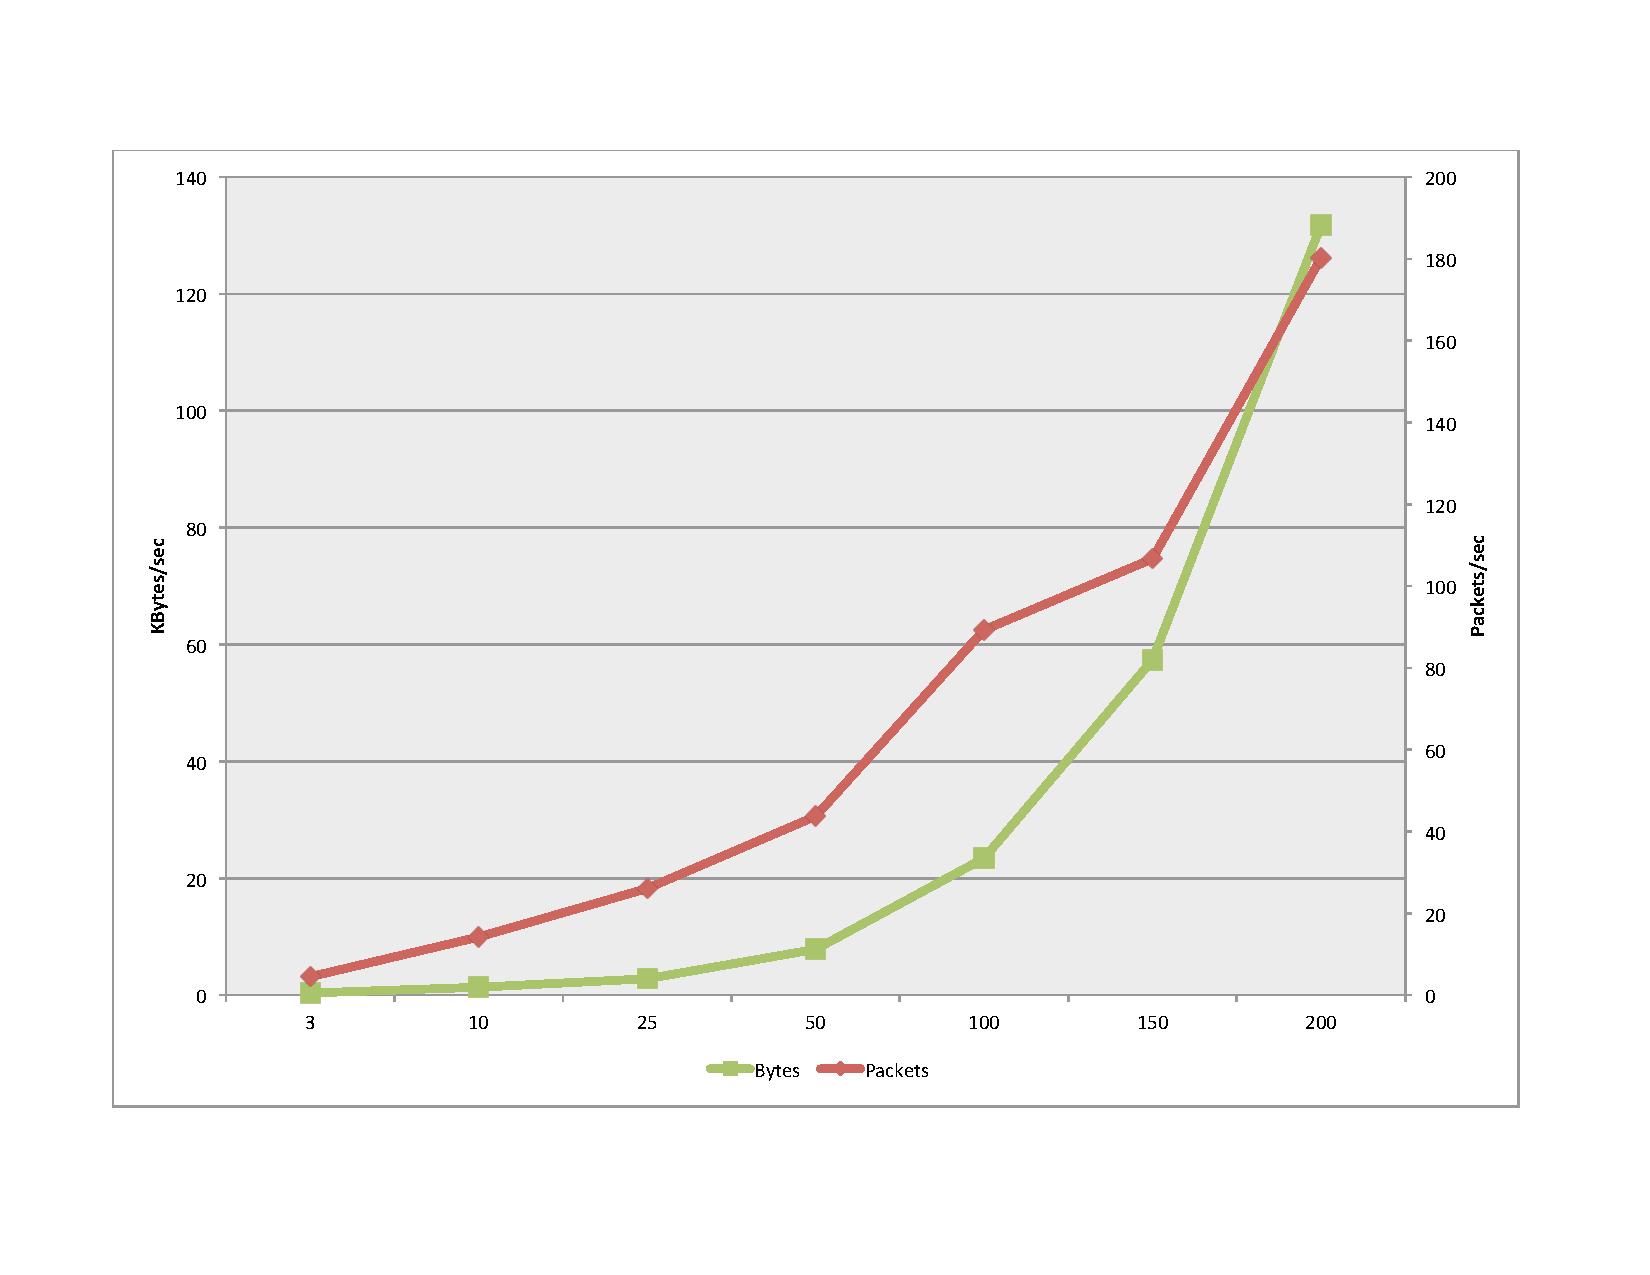
\includegraphics[scale=0.5]{dcamp-net-average.pdf}
    \vspace{-40pt}
    \caption[Scalability: Average Network Utilization]
            {Scalability: Average network utilization as the number of \dcamp nodes increases.}
    \label{fig:net_avg_graph}
\end{figure}

\begin{figure}[H]
    \centering
    \vspace{-20pt}
    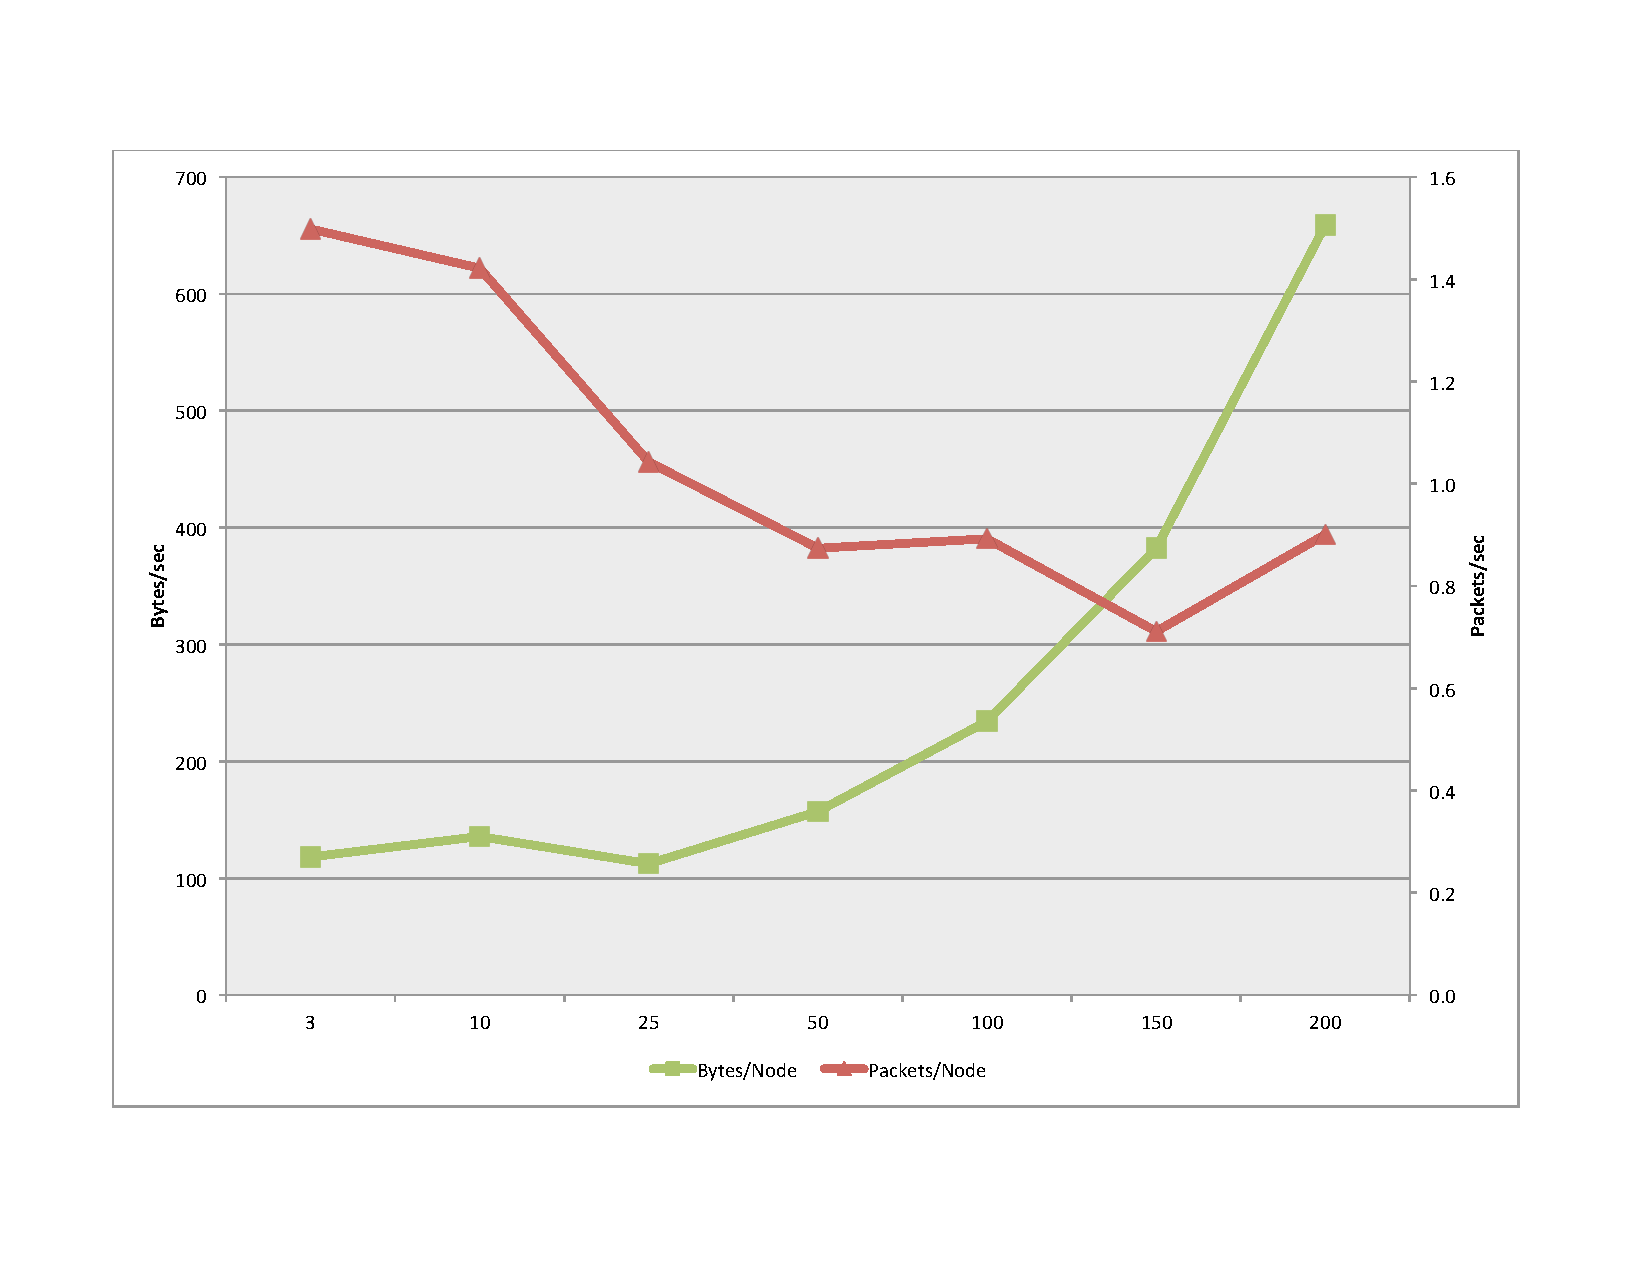
\includegraphics[scale=0.5]{dcamp-net-average-pernode.pdf}
    \vspace{-40pt}
    \caption[Scalability: Average Network Utilization Per Node]
            {Scalability: Average network utilization per node as the number of \dcamp nodes increases.}
    \label{fig:net_avg_pernode_graph}
\end{figure}
